\section{训练目标：让模型在不同预算下学会读视觉记忆}

本章的结论很直接：MemOCR 的视觉画布只有在模型学会“哪里该读、压缩后还能读什么”之后才有价值。训练目标因此围绕两个坐标展开：证据层级，即信息到底是直接决定答案的 \texttt{crucial answer}，还是较低显著性的 \texttt{detail question}；记忆预算，即视觉记忆在最终问答阶段被压到多少 \texttt{image tokens}。

\begin{importantbox}{本章主张}
MemOCR 的训练目标把“证据重要性”和“memory budget”绑定起来：关键证据要能在低预算下从高显著区域被读出，细节事实要能在高清视觉记忆中被精确读出。这个设计让模型同时学习 \texttt{memory drafting} 和 \texttt{memory reading}，也让二维版面的优势变成可训练的能力。
\end{importantbox}

\subsection{两个训练维度：证据层级与记忆预算}

训练的第一条轴是 \texttt{evidence level}。讲者把问题大致拆成两类：一类是高层、总结性、直接影响最终答案的 \texttt{crucial answer}；另一类是较小、较细、视觉显著性较低的 \texttt{detail question}。这一区分非常关键，因为长程推理中最容易混淆的事情是“信息存在”和“信息值得优先保住”。一条事实可能真实存在，却只承担背景作用；另一条事实可能很短，却直接决定答案。

训练的第二条轴是 \texttt{memory budget}。同一张视觉记忆图像可以用较多 \texttt{image tokens} 表示，也可以被压缩到很小的预算。字幕里给出的直观例子是：一张图像可以由 $512$ 个图像 token 表示，也可以被压到 $32$ 或 $64$ 个 token。预算越低，模型看到的图像越粗糙；这相当于把一张清晰白板拍成缩略图，标题还可能读得出来，边角的小字就很容易消失。

\begin{warningbox}{容易混淆的两个预算}
\texttt{memory budget} 指最终回答阶段用于承载记忆状态的预算，常表现为视觉记忆占用的 \texttt{image tokens}；\texttt{context budget} 指模型整次推理可接收的上下文容量。前者是“记忆这张图能占多少空间”，后者是“整次答题纸有多大”。两者相关，却不是同一个量。
\end{warningbox}

用一个教学抽象表示，训练样本可以看成由问题 $Q$、答案 $A$、视觉记忆 $V$、证据层级 $e$ 和预算 $B$ 共同决定：

$$
(Q, A, V, e, B), \qquad e \in \{c, d\}
$$

其中：

\begin{itemize}
    \item $Q$：输入问题，可以要求全局总结，也可以要求读取细节。
    \item $A$：目标答案。
    \item $V$：由 \texttt{renderer} 渲染出来的视觉记忆。
    \item $e=c$：问题依赖 \texttt{crucial evidence}，即关键证据。
    \item $e=d$：问题依赖 \texttt{detail evidence}，即细节证据。
    \item $B$：视觉记忆在最终问答阶段占用的 \texttt{image token} 预算。
\end{itemize}

这个抽象不是论文中的原公式；它的作用是把讲者的二维训练设计写成可检查的结构。第一性原理是：如果信息价值不同，训练样本就应让模型在不同预算下反复面对这种差异。

\begin{figure}[H]
\centering
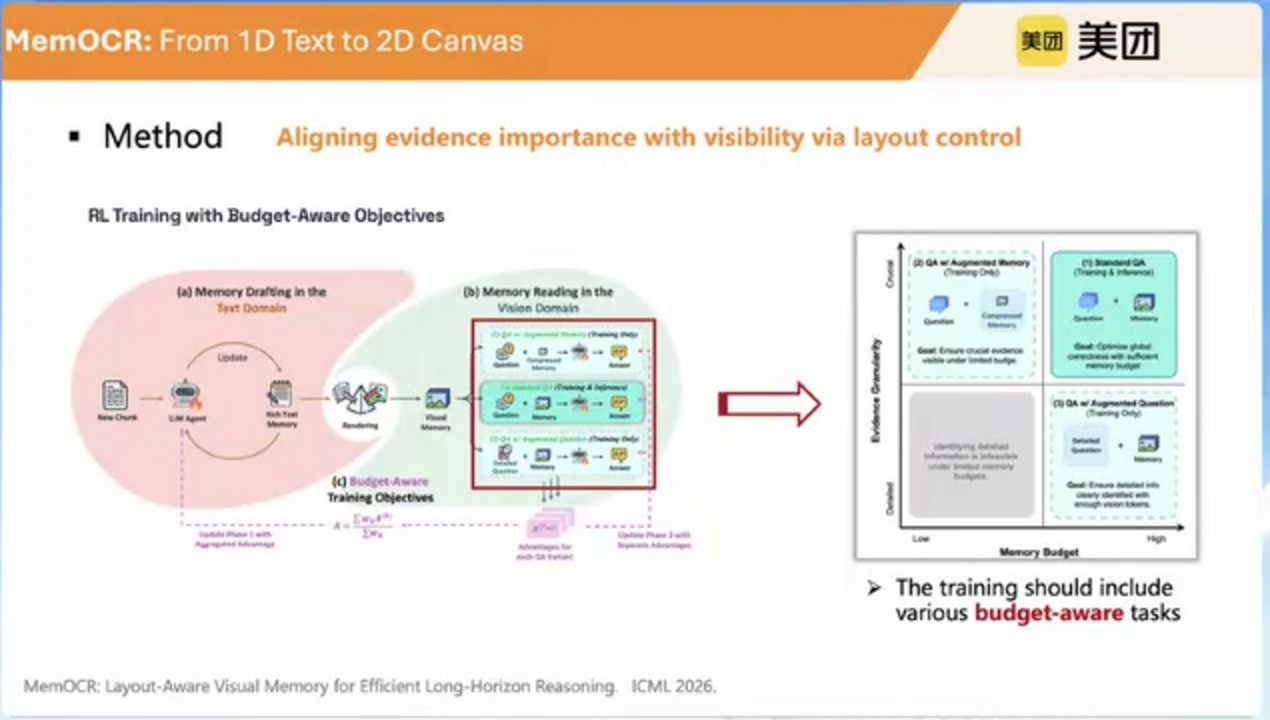
\includegraphics[width=0.86\linewidth,height=0.40\textheight,keepaspectratio]{figures/selected/fig04_budget_aware_training.png}
\caption{预算感知训练目标：左侧展示 \texttt{memory drafting}、渲染与 \texttt{memory reading} 的整体链路，右侧用二维坐标把任务拆成证据粒度与记忆预算两个维度。\protect\footnotemark}
\end{figure}
\footnotetext{视频画面时间区间：00:08:30--00:09:00。}

图中的右侧坐标很重要：纵轴对应问题需要的证据粒度，横轴对应记忆预算。低预算下问全局问题，实际是在逼模型从显著区域读出核心内容；高预算下问细节问题，实际是在检查模型能否读完整张图上的小字和低显著事实。

\subsection{三类数据增强任务}

沿着上述两条轴，MemOCR 构造了三类训练任务。它们的教学意义可以按“先会读整图，再会低预算读重点，最后会高清读细节”理解。

\begin{knowledgebox}{三类训练任务}
\begin{itemize}
    \item \texttt{Standard QA}：使用不经明显压缩的视觉记忆，问题偏向全局认知，训练模型理解完整视觉记忆。
    \item \texttt{Compressed memory + global question}：降低 \texttt{memory budget} 后仍询问全局问题，训练模型从更显著、更被强调的区域读取关键知识。
    \item \texttt{High-resolution memory + detail question}：保持较高图像预算，询问小字或局部细节，训练模型完整读取视觉画布上的低显著信息。
\end{itemize}
\end{knowledgebox}

这三类任务对应三种压力。第一类给模型建立“读视觉记忆”的基本能力；第二类模拟真正部署时的极低预算约束；第三类避免模型只盯标题和大字，丢掉后续推理可能需要的细节。它们合在一起，才让视觉布局承担“优先级编码”的角色。

一个直观类比是复习资料整理。若学生只训练看完整讲义，他可能不会在考前十分钟快速抓重点；若学生只训练看提纲，他又可能找不到小字里的日期、人名和条件。MemOCR 的数据增强把两种能力同时放进训练目标：低预算时像看提纲，高预算时像查原文。

\subsection{联合优化 memory drafting 与 memory reading}

讲者强调三类任务会分别计算 loss，并联合优化 \texttt{memory drafting} 和 \texttt{memory reading} 两个阶段。\texttt{memory drafting} 负责把原始上下文迭代写成副文本记忆；\texttt{memory reading} 负责在视觉域读取渲染后的记忆并回答问题。前者决定“写成什么版面”，后者决定“压缩后是否读得出”。

可以把训练目标写成概念式多任务损失：

$$
\mathcal{L}
= \lambda_0 \mathcal{L}_{\text{standard}}
+ \lambda_c \mathcal{L}_{\text{compressed-global}}
+ \lambda_d \mathcal{L}_{\text{detail-highres}}
$$

其中：

\begin{itemize}
    \item $\mathcal{L}$：总训练损失。
    \item $\mathcal{L}_{\text{standard}}$：普通 QA 任务损失，对应不明显压缩的全局读取。
    \item $\mathcal{L}_{\text{compressed-global}}$：低 \texttt{memory budget} 下回答全局问题的损失。
    \item $\mathcal{L}_{\text{detail-highres}}$：高清视觉记忆下回答细节问题的损失。
    \item $\lambda_0,\lambda_c,\lambda_d$：三类任务的权重。当前字幕与画面没有给出具体数值，因此这里只作为讲义抽象使用。
\end{itemize}

这个损失函数背后的逻辑是因果性的：如果模型在低预算全局问题上失败，它就需要把关键信息写得更显著，或学会从显著区读取；如果模型在高清细节问题上失败，它就需要保留并识别低层级事实。训练不是单纯提高问答准确率，它在塑造一种版面策略。

\begin{warningbox}{关于“16”的两个说法}
字幕在本段附近出现了两个容易混淆的数字：训练中提到过 $16\times$ 压缩率，后续实验中又提到极低预算下的 $16$ 个视觉记忆 token。前者描述压缩倍率，后者描述推理时的记忆 token 数。写作和复核时应把二者分开。
\end{warningbox}

\subsection{本章小结}

MemOCR 的训练设计回答了一个核心问题：视觉记忆怎样从“看起来有层次”变成“模型真的会用”。答案是把证据层级和记忆预算做成训练压力。全局问题要求模型保住关键证据，细节问题要求模型保住局部事实，低预算设置要求模型学会依赖显著区域，高预算设置要求模型仍能读取完整画布。

这一章为下一章的实验结果埋下了因果线索：如果 budget-aware objectives 有效，那么 MemOCR 应该在极低 \texttt{memory budget} 下比文本记忆更稳；如果 layout control 是真正来源，那么把 oracle 证据放入 \texttt{crucial area} 应该比放入 \texttt{detail area} 更有价值。下一章正是对这两个预测的检验。
